% \subsection{Disclaimer}
% \label{sec:disclaimer}
% With this simulation study we will illustrate how easy it is to show
% statistical superiority of any method, if one has enough flexibility in
% changing the simulation conditions and evaluations. We propose a mock-method,
% termed \ainet{}, which seems reasonable at first glance and whose evaluation could actually be
% published in a statistics journal. However, as we will explain in Section~\ref{sec:methods},
% for theoretical reasons the method should actually not be
% superior compared to methods of equal complexity. Throughout this protocol
% we will make a serious attempt at evaluating \ainet{} using state-of-the-art
% simulation study methodology. After the planned simulations
% have been conducted, we will start to apply questionable research practices
% in order to illustrate how easy it is to find simulation conditions and evaluation
% metrics which can make a flawed method look superior.

% \subsection{Introduction}
% \label{sec:introduction}
% The purpose of this protocol is to describe our \emph{a priori} plans for a
% comprehensive simulation study to evaluate the statistical properties of the
% mock-method called adaptive importance elastic net (\ainet) method which is
% described in more detail in Section~\ref{sec:methods}. We will follow the ADEMP
% approach (aims, data-generating process, estimands, methods, performance
% measures) in \citet{Morris2019}. We will plan the simulation study as
% thoroughly as possible. However, in practice there may be difficulties
% and unexpected discoveries which may warrant modifications.
% We will clearly label these as exploratory findings in the analysis.

% \subsection{Timeline}
% \label{sec:timeline}
% Upon writing of this document only some preliminary evaluations have been made:
% After the authors came up with the method on Wednesday 28 July 2021, the method
% was implemented in \textsf{R} and evaluated on the iris data set and a few 
% simulated data sets.
% These analyses showed that for particular choices of hyperparameters, the
% method could sometimes lead to improved predictive performance compared to
% standard and L1-penalized logistic regression. However, in many cases
% performance was actually equal or worse.

% We then started to write the simulation protocol. All versions of the protocol are
% available on the GitHub repository (\url{https://github.com/SamCH93/SimPaper}),
% the final version will be time\-stamped and tagged. As discussed in
% Section~\ref{sec:performance}, some preliminary simulation runs will be conducted
% to estimate the number of simulations needed to ensure a sufficiently small Monte
% Carlo error. The test run will also be used to assess whether there are severe
% convergence problems and if so, the simulation parameters may be modified 
% (Section~\ref{sec:exceptions}). This milestone will also be time\-stamped.

%%%%%%%%%%%%%%%%%%%%%%%%%%%%%%%%%%%%%%%%%%%%%%%%%%%%%%%%%%%%%%%%%%%%%%%%%%%%%%%%
\subsection{Aims} \label{sec:aims}
%%%%%%%%%%%%%%%%%%%%%%%%%%%%%%%%%%%%%%%%%%%%%%%%%%%%%%%%%%%%%%%%%%%%%%%%%%%%%%%%

The aim of this simulation study is to systematically study the predictive
performance of \ainet{} for a binary prediction task. The simulation conditions
should resemble typical conditions found in the development of prediction models
in biomedical research. In particular we want to evaluate the performance of
\ainet{} conditional on
\begin{itemize}
  \item low- and high-dimensional covariates
  \item (un-)correlated covariates
  \item small and large sample sizes
  \item varying baseline prevalences
\end{itemize}
\ainet{} will be compared to other (penalized) binary regression models
from the literature, namely
\begin{itemize}
  \item Binary logistic regression: the simplest and most popular method for
        binary prediction
  \item Elastic net: a generalization of LASSO and ridge regression, the most
        widely used penalized regression methods
  \item Adaptive elastic net: a generalization of the most popular weighted 
  penalized regression method (adaptive LASSO)
  \item Random forest: a popular, more flexible method. This method is related to
        \ainet{}, see Section~\ref{sec:methods}.
\end{itemize}
These cover a wide range of established methods with varying flexibility and
serve as a reasonable benchmark for \ainet. There are many more extensions of
the adaptive elastic net in the literature \citep[see \eg{} the review by][]{Vidaurre2013}.
However, most of these extensions focus on variable selection and
estimation instead of prediction, which is why we restrict our focus only on the
four methods above.

%%%%%%%%%%%%%%%%%%%%%%%%%%%%%%%%%%%%%%%%%%%%%%%%%%%%%%%%%%%%%%%%%%%%%%%%%%%%%%%%
\subsection{Data-generating process} \label{sec:dgp}
%%%%%%%%%%%%%%%%%%%%%%%%%%%%%%%%%%%%%%%%%%%%%%%%%%%%%%%%%%%%%%%%%%%%%%%%%%%%%%%%

In each simulation $b = 1, \dots, B$, we generate a data set consisting of $n$
realizations, \ie $\{(\ry_i, \rx_i)\}_{i=1}^n$. A datum $(\rY, \rX)$ consists of
a binary outcome $\rY \in \{0, 1\}$ and $p$-dimensional covariate vector
$\rX \in \RR^p$. The binary outcomes are generated by
\begin{align*}
  Y \given \rx &\sim \BD\left(\expit\left\{\beta_0 +
	\rx^\top\shiftparm\right\}\right)
\end{align*}
with $\expit(z) = (1 + \exp(-z))^{-1}$ and the covariate vectors are generated by
\begin{align*}
  \rX &\sim \ND_p\left(0, \Sigma\right)
\end{align*}
with covariance matrix $\Sigma$ that may vary across simulation conditions (see below).
The baseline prevalence is $\prev = \expit(\beta_0)$. The coefficient vector
$\shiftparm$ is generated from
\begin{align*}
  \shiftparm \sim \ND_p(0, \Id)
\end{align*}
once per simulation. Finally, the simulation parameters are varied
fully factorially (except for the removal of some unreasonable conditions) as described below, leading to a total of 128
scenarios, see below.

\subsection*{Sample size}
The sample size used in the development of predictions models varies widely
\citep{Damen2016}. We will use $n \in \{100, 500, 1000, 5000\}$, which span typical values
occurring in practice. Note that previous simulation studies usually chose sample
size based on the implied number of events together with the number of covariates
in the model for easier interpretation \citep{vanSmeden2018, Riley2018}. We will use this approach in
reverse to determine the dimensionality of the parameters below.

\subsection*{Dimensionality}
Previous simulation studies showed that events per variable ($\EPV$) rather than the absolute sample
size $n$ and dimensionality $p$ influences the predictive performance of a
method. We will therefore define the dimensionality $p$ via EPV
by $$p = \frac{n \cdot \prev}{\EPV}$$ and $2 \leq p \leq 100.$ If the
above formula gives non-integer values, the next larger integer will be used for
$p$. When the formula gives values above 100 or below 2, this simulation
condition will be removed from the design. This is done because prediction
models are in practice only multivariable models ($p \geq 2$), but at the same
time the number of predictors is rarely larger than $p \geq 100$
\citep{Kreuzberger2020,Seker2020, Wynants2020}. The exception are studies
considering complex data, such as images, omics, or text data which are not the
focus here. The values $\EPV \in \{20, 10, 1, 0.5\}$ are chosen to cover scenarios
with small to large number of covariates \citep[\cf][]{vanSmeden2018}.

% \subsection*{Sparsity in $\shiftparm$}
% We consider sparse and dense simulation settings for $\shiftparm$. We choose
% sparsity of $\shiftparm$ based on the consistency requirement for the LASSO
% \citep[Ch. 2.4.2]{buhlmann2011statistics}, \ie
% $$q = \begin{cases}
  % \floor{\sqrt{n/\log p}} & p > 1 \\
  % 0 & p \leq 1,
% \end{cases}$$
% so $q$ will depend on the sample size
% $n$ and the number of covariates $p$ ( determined via the EPV).
% In the simulations where $\shiftparm$ is dense, we set $q = p$.

\subsection*{Collinearity in $\rX$}
We distinguish between no, low, medium and high collinearity. The diagonal
elements of $\Sigma$ are given by $\Sigma_{ii} = 1$ and the off-diagonal
elements are set to $\Sigma_{ij} = \rho$, $\rho \in \{0, 0.3, 0.6, 0.95\}$.
These values cover the typical (positive) range of correlations.

\subsection*{Baseline prevalence}
Different baseline prevalences $\expit(\beta_0) \in \{0.01, 0.05, 0.1\}$ are 
considered, reflecting a reasonable range of prevalences for rare to
common diseases/adverse events.

\subsection*{Test data}
In order to test the out-of-sample predictive performance, we generate a test data set of
$n_{\text{test}} = 10000$ data points in each simulation $b$.

%%%%%%%%%%%%%%%%%%%%%%%%%%%%%%%%%%%%%%%%%%%%%%%%%%%%%%%%%%%%%%%%%%%%%%%%%%%%%%%%
\subsection{Estimands} \label{sec:estimands}
%%%%%%%%%%%%%%%%%%%%%%%%%%%%%%%%%%%%%%%%%%%%%%%%%%%%%%%%%%%%%%%%%%%%%%%%%%%%%%%%
We will estimate different quantities to evaluate overall predictive performance,
calibration, and discrimination, respectively. All methods will be evaluated on
independently generated test data.

\subsubsection{Primary estimand}

\begin{itemize}
  \item \textbf{Brier score.} We compute the Brier score as
  $$\BS = n_{\text{test}}^{-1} \sum_{i=1}^{n_{\text{test}}} (y_{i} - \hat{y}_{i})^2,$$
  where $\hat{y} = \widehat\Prob(Y = 1 \given \rx)$.
  Lower values indicate better predictive performance in terms of calibration and
  sharpness. A prediction is well-calibrated if the observed proportion
  of events is close to the predicted probabilities. Sharpness refers to how
  concentrated a predictive distribution is (\eg{} how wide/narrow a prediction interval is),
  and the predictive goal is to maximize sharpness subject to calibration
  \citep{Gneiting2008}.
  The Brier score is a proper scoring rule, meaning that it is minimized if a
  predicted distribution is equal to the data-generating distribution
  \citep{Gneiting2007}. Proper scoring rules thus encourage honest
  predictions. The Brier score is therefore a principled choice for our primary estimand.
\end{itemize}

\subsubsection{Secondary estimands}
\begin{itemize}
  \item \textbf{Scaled Brier score.} The scaled Brier score (also known as Brier skill score) is computed as
  $$\BS^{*} = 1 - \BS/\BS_{0}$$
  with $\BS_{0} = \bar{y}(1 - \bar{y})$ and $\bar{y}$ the observed prevalence in
  the data set. The scaled Brier score takes into account that the
  prevalence varies across simulation conditions. Hence, the scaled Brier score
  can be compared between conditions \citep{Schmid2005, steyerberg2019clinical}.

  \item \textbf{Log-score.} We compute the log-score on independently generated test data,
  $$\LS = - n_{\text{test}}^{-1} \sum_{i=1}^{n_{\text{test}}} \left\{ y_{i} \log(\hat{y}_{i})
  + (1 - y_{i}) \log (1 - \hat{y}_{i})\right\},$$
  will be used as a secondary measure of overall predictive performance. Lower
  values indicate better predictive performance in terms of calibration and
  sharpness. The log-score is a strictly proper scoring rule, however, it is more
  sensitive to extreme predicted probabilities compared to the Brier score \citep{Gneiting2007}.
  
  \item \textbf{AUC.} The AUC is given by
  $$\text{AUC} = \max\{\text{PI}, 1 - \text{PI}\}$$
  with $$\text{PI} =  
  \widehat\Prob(Y_i \geq Y_j \given \rx_i, \rx_j), \; i,j = 1, \dots, n_{\text{test}},$$
  where $Y_i$ and $Y_j$ denote case and non-case, respectively. The AUC is related
  to the area under the receiver-operating-characteristic (ROC) curve \citep{steyerberg2019clinical}.
  It will be used as a measure of discrimination and values closer to one
  indicate better discriminative ability. Discrimination describes the ability
  of a prediction model to discriminate between cases and non-cases.
  Other discrimination measures, such as accuracy, sensitivity, specificity, etc.,
  are not considered because we want to evaluate predictive performance
  in terms of probabilistic predictions instead of point predictions/classification.

  \item \textbf{Calibration slope $\hat b$.}  
  The calibration slope $\hat b$ is obtained by regressing
  the test data outcomes $y_{\text{test}}$ on the models' predicted logits $\logit({\hat{y}})$,
  \ie
  $$\logit\Ex[Y \given \hat\ry] = a + b\logit(\hat\ry).$$
  This measure will be used to assess calibration and deviations of $\hat b$ from
  one indicate miscalibration \citep{steyerberg2019clinical}.

  \item \textbf{Calibration in the large $\hat a$.} We inspect calibration in the
  large $\hat a$ on independently generated test data, from the model
  $$\logit\Ex[Y \given \hat\ry] = a + \logit(\hat{y}).$$
  This measure will also be used to assess calibration and deviations of $\hat a$ from
  zero indicate miscalibration \citep{steyerberg2019clinical}.
\end{itemize}

To facilitate comparison between simulation conditions, all estimands will also
be corrected by the oracle version of the estimand, \eg{} the Brier score will be
computed from the ground truth parameters and the simulated data $\rx$,
subsequently the oracle Brier score will be subtracted from the estimated
Brier score.

%%%%%%%%%%%%%%%%%%%%%%%%%%%%%%%%%%%%%%%%%%%%%%%%%%%%%%%%%%%%%%%%%%%%%%%%%%%%%%%%
\subsection{Methods} \label{sec:methods}
%%%%%%%%%%%%%%%%%%%%%%%%%%%%%%%%%%%%%%%%%%%%%%%%%%%%%%%%%%%%%%%%%%%%%%%%%%%%%%%%

\subsubsection{\ainet}
We now present the mock-method and give a superficial motivation why it could
lead to improved predictive performance:
Choosing the vector of penalization weights in the adaptive LASSO becomes difficult
in high-dimensional settings. For instance, using absolute LASSO estimates as penalization
weights omits the importance of several predictors by not selecting them, 
especially in the case of highly correlated predictors \citep{Algamal2015}.
The adaptive importance elastic net (\ainet{}) circumvents this problem by
employing a random forest to estimate the
penalization weights via an \emph{a priori} chosen variable importance measure.
In this way, the importance of all variables enter the penalization weights simultaneously.

The penalized log-likelihood for \ainet{} for a single observation $(\ry, \rx)$
is defined as
$$\ell_{\text{AINET}}(\beta_0, \shiftparm; \ry, \rx, \alpha, \lambda, \wvec) = 
  \ell(\beta_0, \shiftparm; \ry, \rx) + \aipen$$
where
$$\ell(\beta_0, \shiftparm; \ry, \rx) = 
  \ry \log\left(\expit\left\{\beta_0 + \linpred\right\}\right)
  + (1 - \ry) \log\left(1 - \expit\left\{\beta_0 + \linpred\right\}\right)$$
denotes the log-likelihood of a binomial GLM and
$\wvec$ is derived from a random forest variable importance measure $\IMP$ as
$$w_j = 1 - \left(\frac{\IMP_j}{\sum_{k=1}^p \IMP_k}\right)^\gamma,$$
where we transform $\IMP$ to be non-negative via
% $$\IMP = \widetilde\IMP - \min_j\{\widetilde{\IMP}_j\},$$
% or
$$\IMP_j = \max\{0, \widetilde\IMP_j\}$$
and $\gamma$ is a hyperparameter for the influence of the weights similar to
$\gamma$ hyperparameter of the adaptive elastic net.
\ainet{} is fitted by maximizing its penalized log-likelihood assuming i.i.d.
observations $\{(\ry_i, \rx_i)\}_{i=1}^n$, \ie
$$\arg\max_{\beta_0, \shiftparm} \sum_{i = 1}^n \ell_{\text{AINET}}(\beta_0,
\shiftparm; \ry_i, \rx_i, \alpha, \lambda, \wvec).$$

Per default, we choose mean decrease in the Gini coefficient for $\widetilde\IMP$.
Hyperparameters of the random forest are not tuned, but kept at their default
values (\eg{} \code{mtry}, \code{ntree}). The hyperparameter $\gamma = 1$ will stay
constant for all simulations.

\ainet{} is supposed to seem like a reasonable method at first glance. However, 
\ainet{} cannot be expected to share desirable theoretical properties with the 
usual adaptive LASSO, such as oracle estimation \citep{Zou2006}. This is because 
the penalization weights $\wvec$ do not meet the required consistency assumption. 
Also in terms of prediction performance, \ainet{} is not expected to outperform 
methods of comparable complexity.

\subsubsection{Benchmark methods}

\begin{itemize}
   \item \textbf{Binary logistic regression} \citep{mccullagh2019generalized} 
   with and without ridge penalty for high- and
   low-dimensional settings, respectively. In case a ridge penalty is needed,
   it is tuned via 5-fold cross-validation by following the ``one standard
   error'' rule as implemented in \pkg{glmnet} \citep{Friedman2010}. 
   \item \textbf{Elastic net} \citep{Zou2005}, for which the penalized 
   log-likelihood is given by
    $$\ell_{\text{EN}}(\beta_0, \shiftparm; \ry, \rx, \alpha, \lambda) = 
      \ell(\beta_0, \shiftparm; \ry, \rx) + \llpen.$$
    Here, $\alpha$ and $\lambda$ are tuned via 5-fold cross-validation by following 
    the ``one standard error'' rule.
   \item \textbf{Adaptive elastic net} \citep{Zou2006}, with penalized loss function
    $$\ell_{\text{adaptive}}(\beta_0, \shiftparm; \ry, \rx, \alpha, \lambda, \wvec)
    = \ell(\beta_0, \shiftparm; \ry, \rx) + \aipen.$$
    Here, the penalty weights $\wvec$ are inverse coefficient estimates from a
    binary logistic regression
    $$\hat{w}_j = \lvert\hat\eparm_j\rvert^{-\gamma},$$
    where $\lambda$ and $\alpha$ are tuned via 5-fold cross-validation by 
    following the ``one standard error'' rule.
    The hyperparameter $\gamma = 1$ will stay constant for all simulations.
    In case $p > n$, we estimate the penalty weights using a ridge penalty, tuned
    via an additional nested 5-fold cross-validation
    by following the ``one standard error'' rule.
    \item \textbf{Random forests} \citep{Breiman2001} for binary outcomes without 
    hyperparameter tuning. The default parameters of \pkg{ranger} will be used 
    \citep{ranger2017}. % , \ie
    % \code{ntree = 500}, \code{mtry = floor(sqrt(p))}, \code{min.node.size = },
    % \code{max.depth = }, \code{sample.fraction = }
\end{itemize}


%%%%%%%%%%%%%%%%%%%%%%%%%%%%%%%%%%%%%%%%%%%%%%%%%%%%%%%%%%%%%%%%%%%%%%%%%%%%%%%%
\subsection{Performance measures} \label{sec:performance}
%%%%%%%%%%%%%%%%%%%%%%%%%%%%%%%%%%%%%%%%%%%%%%%%%%%%%%%%%%%%%%%%%%%%%%%%%%%%%%%%

The distribution of all estimands from Section~\ref{sec:estimands} will be
assessed visually with box- and violin-plots that are stratified by method and
simulation conditions. We will also compute mean, median, standard deviation,
interquartile range, and 95\% confidence intervals
% \begin{itemize}
  % \item Mean
  % \item Median
  % \item Standard deviations
  % \item Interquartile range
  % \item 95\% confidence intervals
% \end{itemize}
for each of the estimands. Moreover, instead of ``eye-balling'' differences in predictive
performance across methods and conditions, we will formally assess them by regressing
the estimands on the method and simulation conditions \citep[\cf][]{Skrondal2000}.
To do so, we will use
a fully interacted model with the interaction between the methods and the
128 simulations conditions, \ie in R notation:
\texttt{estimand $\sim$ 0 + method:scenario}. %sample\_size:dimensionality:sparsity:colinearity:prevalence}
We will rank pairwise comparison between two methods within a single condition
by their $p$-values, to more easily identify conditions where methods
show differences in predictive performance. The choice of a significance level
at which a method is deemed superior will be determined based on preliminary
simulations. We set this level to 5\%, where $p$-values will be adjusted using
the single-step method \citep{pkg:multcomp} within a single simulation condition
for comparisons between \ainet{} and any other method.


\subsection{Determining the number of simulations}

We determine the number of simulation $B$ such that the Monte Carlo
standard error of the primary estimand, the mean Brier score $\BS/B$,
is sufficiently small. The variance of $\BS/B$ is given by
\begin{align*}
  \Var\left(\BS/B\right)
  &= \frac{\Var\left\{(y -
    \hat{y})^{2}\right\}}{B \cdot n_{\text{test}}}
  % &= B^{-1}n_{\text{test}}^{-1} \left\{\Ex[(y_{ib} - \hat{y}_{ib})^{4}] -
  %   \Ex[(y_{ib} - \hat{y}_{ib})^{2}]^{2}\right\}
\end{align*}
and $\Var\left\{(y_{ib} - \hat{y}_{ib})^{2}\right\}$ could be decomposed further
\citep{Bradley2008}. However, the resulting expression is difficult to evaluate
for our data-generating process as it depends on several of the simulation
parameters. We therefore follow a similar approach as in \citet{Morris2019} and
estimate $\widehat{\Var}\left\{(y_{ib} - \hat{y}_{ib})^{2}\right\} < V$ from an
initial small simulation run with 100 simulations per condtion to get an upper
bound $V$ for worst-case variance across all simulation conditions.
Therefore, the number of simulations is then given by
$$B = \frac{V}{n_{\text{test}} \Var\left(\BS\right)}.$$
Since $\BS \in [0, 1]$ we decide that we require the Monte Carlo standard error
of $\BS$ to be lower than four significant digits, $0.0001$.

The initial simulation run led to an estimated worst case variance of
$\widehat{V} = 0.2$. Therefore, we compute that
$$B = 0.2/(10000 \times 0.0001^{2}) = 2000$$
replications are required to obtain Brier score estimates with the
desired precision.

%%%%%%%%%%%%%%%%%%%%%%%%%%%%%%%%%%%%%%%%%%%%%%%%%%%%%%%%%%%%%%%%%%%%%%%%%%%%%%%%
\subsection{Handling exceptions} \label{sec:exceptions}
%%%%%%%%%%%%%%%%%%%%%%%%%%%%%%%%%%%%%%%%%%%%%%%%%%%%%%%%%%%%%%%%%%%%%%%%%%%%%%%%
It is inevitable that convergence issues and other problems will arise
in the simulation study. We will handle them as follows:
\begin{itemize}
  \item If a method fails to converge, the simulation will be excluded from the
  analysis. The failing simulations will not be replaced with new simulations that
  successfully converge as convergence may be impossible for some scenarios.
  \item We will report the proportion of simulations with convergence issues
  for each method and discuss the potential reasons for their emergence.
  \item In case of severe convergence issues or other problems (more than 10\% of the
  simulations failing within a setting), we may adjust
  the simulation parameters post hoc. This will be indicated in the discussion of
  the results.
  \item Convergence may be possible for certain tuning parameters of a method
  (\eg{} cross-validation of LASSO may fail for some values $\lambda$ while it could
  work for others). In this case we will choose a parameter value where the method
  still converges, as one would usually do with a real data set.

\end{itemize}


% %%%%%%%%%%%%%%%%%%%%%%%%%%%%%%%%%%%%%%%%%%%%%%%%%%%%%%%%%%%%%%%%%%%%%%%%%%y%%%%%%
% \subsection{Software} \label{sec:software}
% %%%%%%%%%%%%%%%%%%%%%%%%%%%%%%%%%%%%%%%%%%%%%%%%%%%%%%%%%%%%%%%%%%%%%%%%%%%%%%%%

% The simulation study is conducted in the \textsf{R} language for statistical
% computing \citep{pkg:base} using the version
% % R.version$version.string
% 4.1.1.
% \ainet{} is implemented in the \pkg{ainet} package and available on GitHub 
% (\url{https://github.com/SamCH93/SimPaper}).
% We use \pkg{pROC} version 1.18.0 to compute the AUC \citep{pkg:proc}.
% Random forests are fitted using \pkg{ranger} version 0.13.1 \citep{ranger2017}.
% For penalized likelihood methods, we use \pkg{glmnet} version 4.1.2
% \citep{Friedman2010,Simon2011}.
% The \pkg{SimDesign} package version 2.7.1 is used to set up simulation scenarios
% \citep{Chalmers2020}.

% %%%%%%%%%%%%%%%%%%%%%%%%%%%%%%%%%%%%%%%%%%%%%%%%%%%%%%%%%%%%%%%%%%%%%%%%%%%%%%%%
% \subsection{Preliminary simulations}
% %%%%%%%%%%%%%%%%%%%%%%%%%%%%%%%%%%%%%%%%%%%%%%%%%%%%%%%%%%%%%%%%%%%%%%%%%%%%%%%%

% In the following we report the results of the preliminary simulation study which
% was used to plan the size of the full simulation. We report convergence issues,
% errors, warnings, and any amendments that were made to the protocol.

% \subsubsection{Results}

% Figure~\ref{fig:tiebrier2} displays the results for the difference in Brier scores
% between \ainet{} and all other methods. Confidence intervals are adjusted within
% a simulation condition, because each simulation run is independent. The adjustment
% is based on the single-step method using the \pkg{multcomp} package \citep{pkg:multcomp}.
% We show only the results for the primary estimand.

% % ------------------------------------------------------------------------------
% \begin{landscape}
% \begin{figure}[!ht]
% \center
% 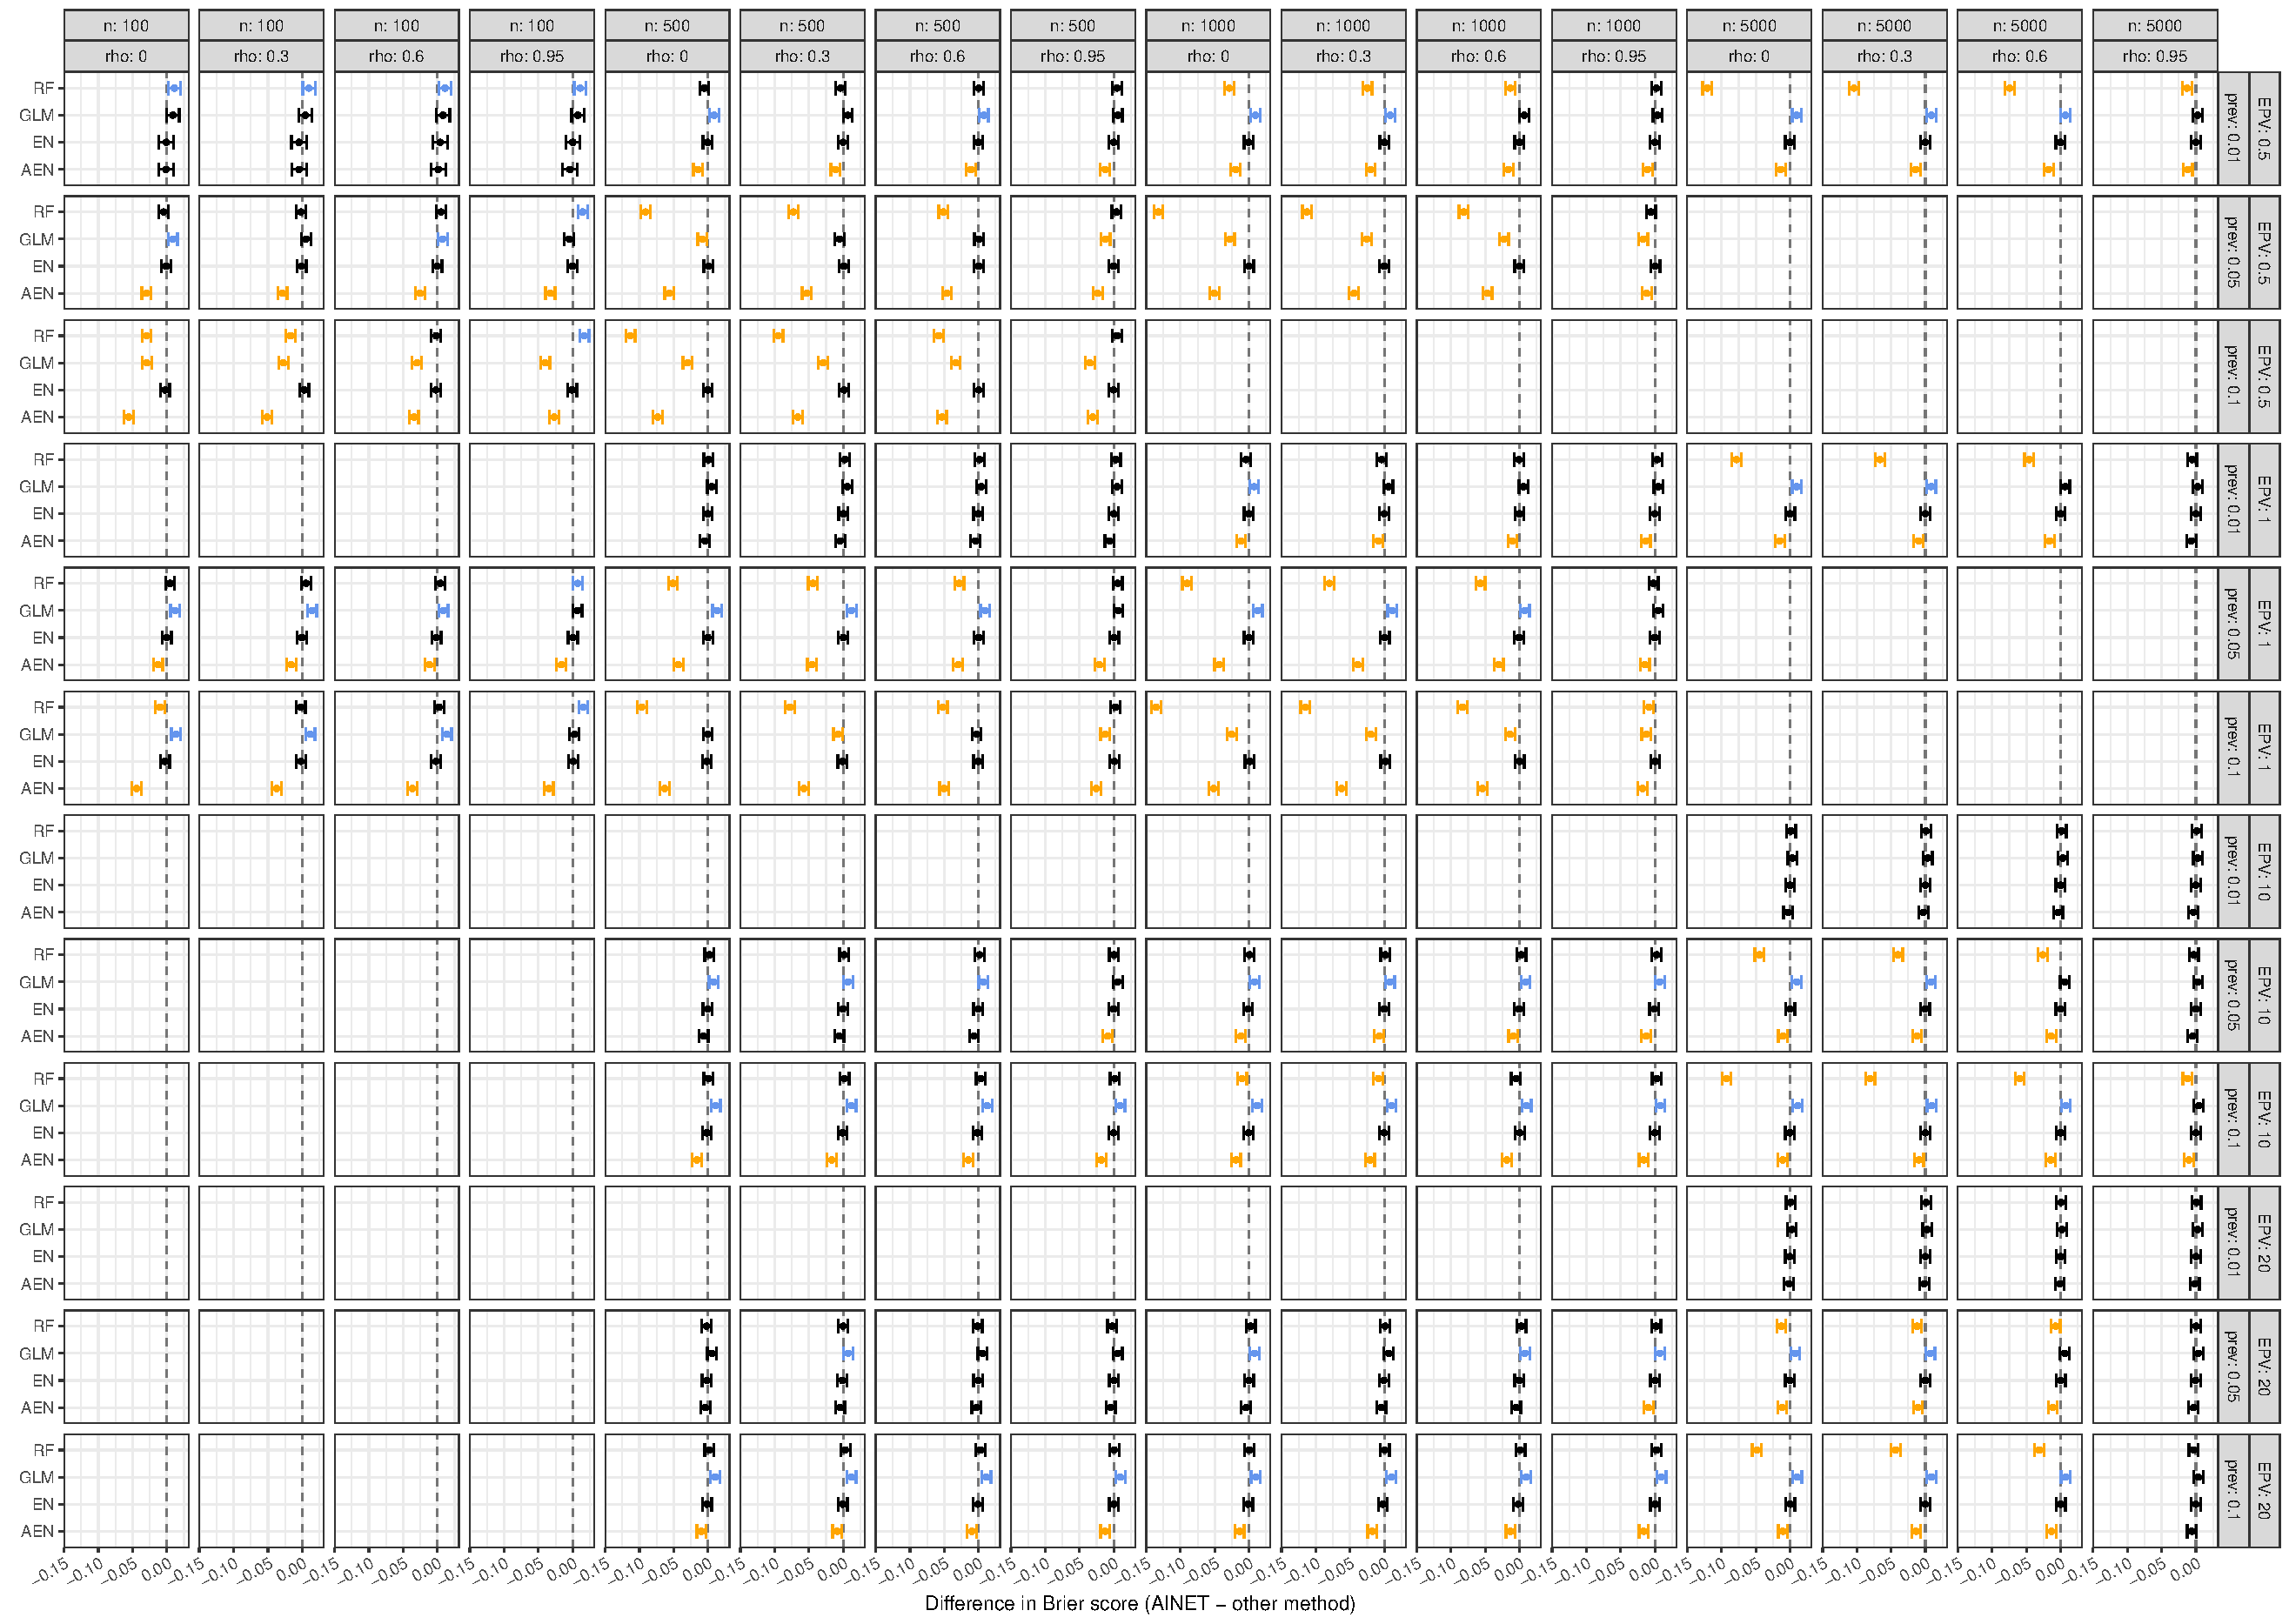
\includegraphics[width=0.9\linewidth]{figures-appendix/figures-protocol/tie-fighter_brier.pdf}
% \caption{Tie-fighter plot for the difference in Brier score between any method
%   on the $y$-axis and \ainet{}. Empty facets correspond to simulation conditions
%   for which $p < 1$ or $p > 100$. Confidence intervals are colored according to
%   significance at the 5\% level, indicating a better (negative difference), neutral
%   (including zero), or worse (positive difference) performance of \ainet{}.} \label{fig:tiebrier2}
% \end{figure}
% \end{landscape}
% % ------------------------------------------------------------------------------

% \subsubsection{Convergence issues}

% Figure~\ref{fig:failures} reports the proportion of simulations with convergence 
% issues. As outlined in Section~\ref{sec:exceptions},
% scenarios in which the proportion of simulations with convergence issues exceeds 
% $> 10\%$ warrant a closer look.

% Most convergence issues seem to arise for low sample size ($n = 100$) and low
% prevalence ($\prev < 0.05$). This leads to a low number of cases and therefore
% problems with the methods that use cross-validation. We decided to still run
% this simulation condition and just exclude the non-converged observations and
% in the end report the proportion of simulations that fail.

% % ------------------------------------------------------------------------------
% \begin{landscape}
% \begin{figure}[!ht]
% \center
% 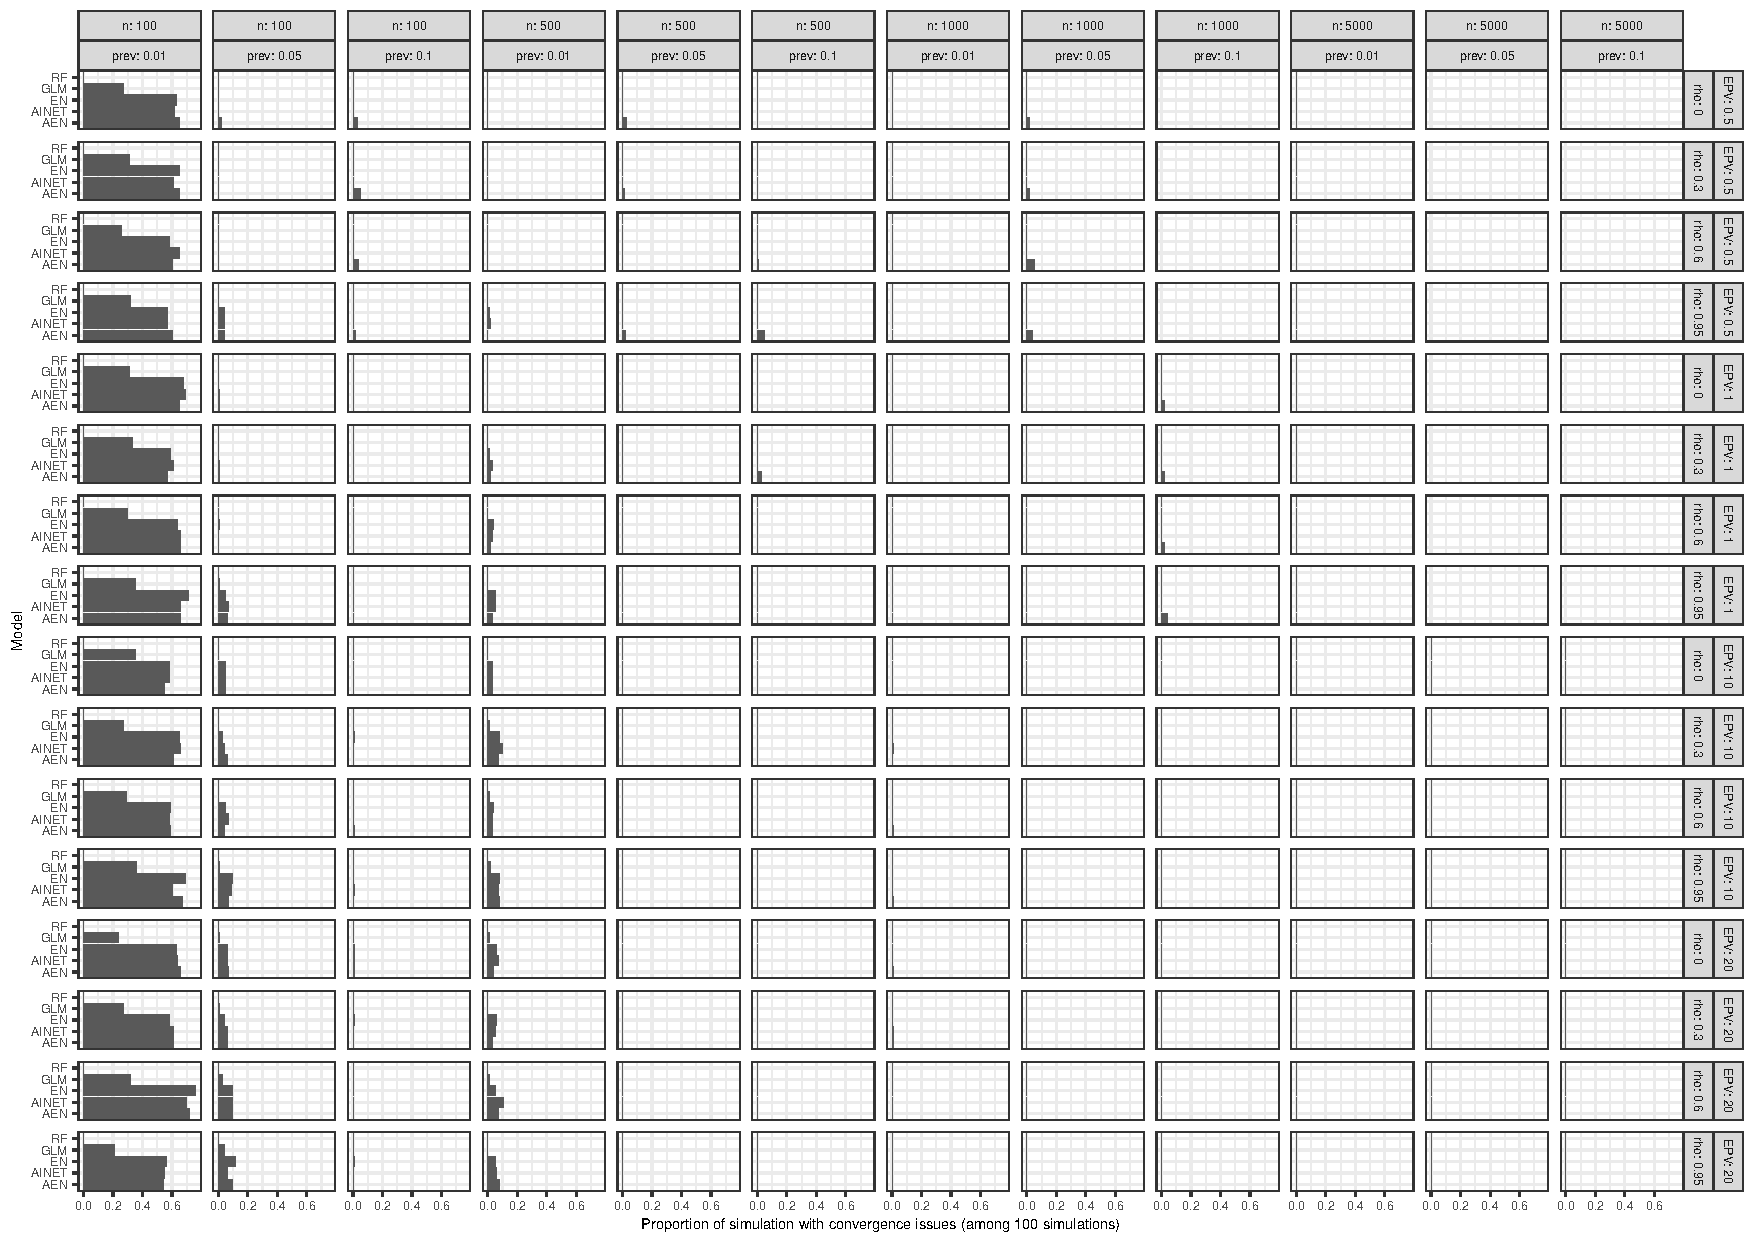
\includegraphics[width=0.9\linewidth]{figures-appendix/figures-protocol/failed.pdf}
% \caption{Simulations with convergence issues.} \label{fig:failures}
% \end{figure}
% \end{landscape}
% % ------------------------------------------------------------------------------

% \subsubsection{Errors}

% Errors which terminated the whole simulation run only occurred in case no events
% were present in the training data (see Figure~\ref{fig:errors}), which happened
% only for low sample size ($n = 100$) and low prevalence ($\prev < 0.05$).
% In practice no model could be fitted for such a scenario, which is why they are
% dropped entirely from the analysis.

% % ------------------------------------------------------------------------------
% \begin{figure}[!ht]
% \center
% 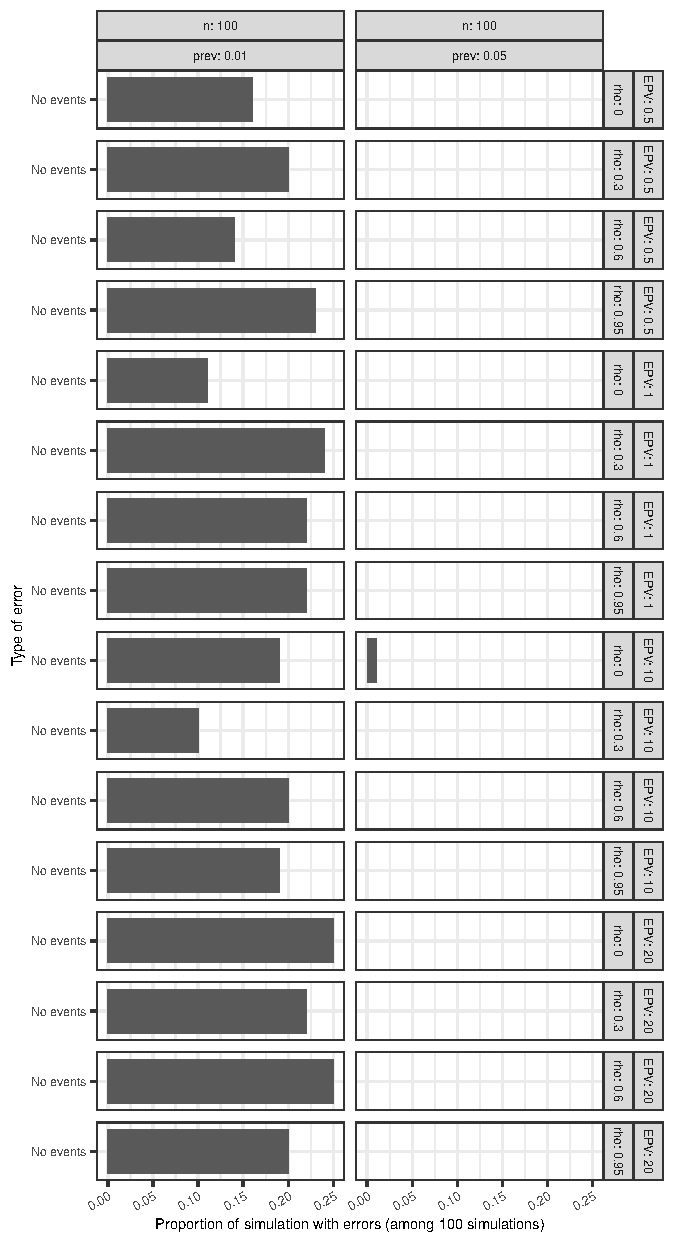
\includegraphics[width=0.7\textwidth]{figures-appendix/figures-protocol/errors.pdf}
% \caption{Simulation runs which were terminated due to an error.} \label{fig:errors}
% \end{figure}
% % ------------------------------------------------------------------------------

% \subsubsection{Warnings}

% Several different warnings were observed in the preliminary simulations, namely
% (i) a too low number of events, (ii) over-confident zero/one predictions of the
% random forest, (iii) \code{cv.glmnet()} convergence issues for a particular $\lambda$,
% and (iv) an empty model being returned (\ie no non-zero coefficients).
% Figure~\ref{fig:warnings} summarizes the occurrence of each warning over all
% scenarios.

% % ------------------------------------------------------------------------------
% \begin{landscape}
% \begin{figure}[!ht]
% \center
% 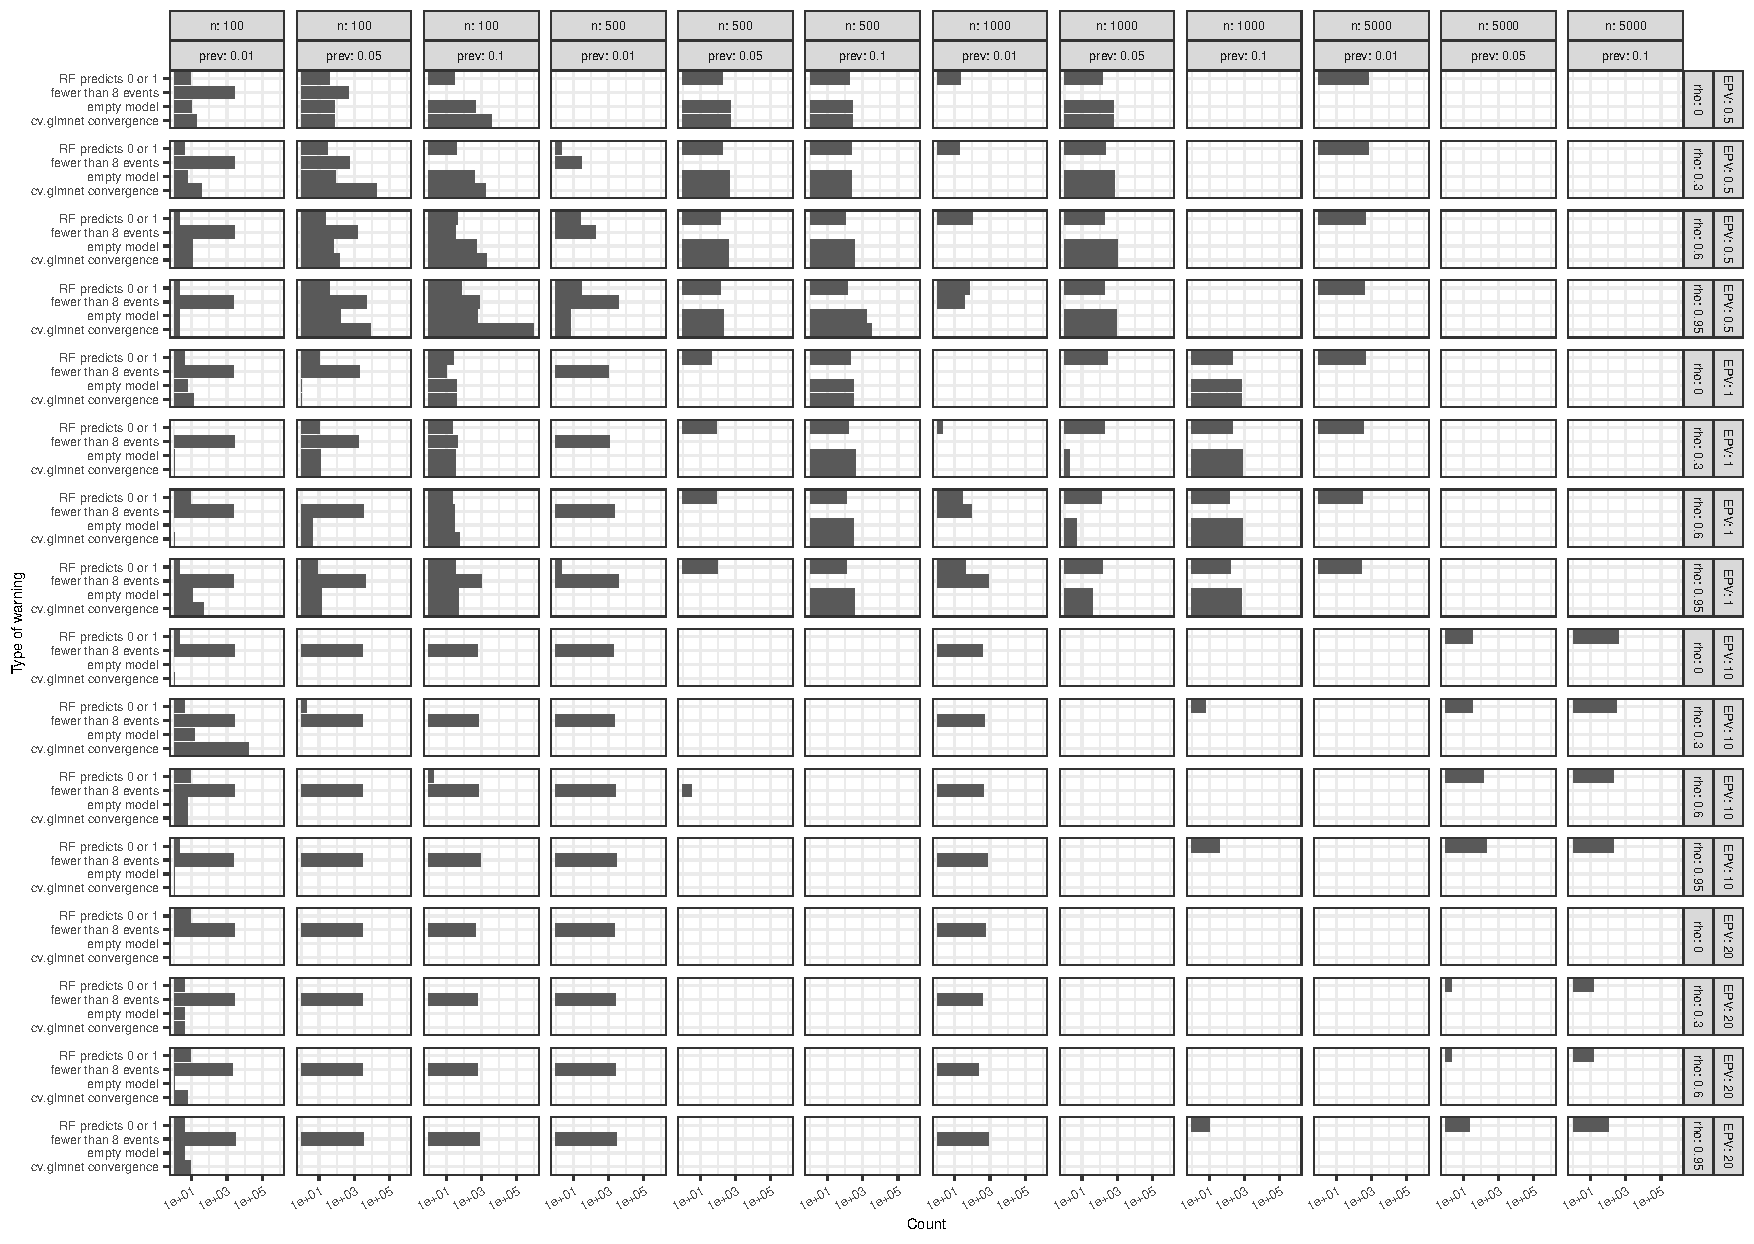
\includegraphics[width=0.9\linewidth]{figures-appendix/figures-protocol/warnings.pdf}
% \caption{Warning messages across all simulation runs, conditions, and methods.} \label{fig:warnings}
% \end{figure}
% \end{landscape}
% % ------------------------------------------------------------------------------

% \subsubsection{Deviations}

% % ------------------------------------------------------------------------------
% \begin{table}[!ht]
% \center
% \caption{Changes compared to the previous version of the protocol.} \label{tab:deviations}
% \begin{tabular}{p{0.3\textwidth}p{0.6\textwidth}}
%   \toprule
%   \textbf{Deviation} & \textbf{Justification} \\
%   \midrule
%   Remove high-dimensional conditions
%                      & We decided to remove all conditions involving
%                       $p > 100$ because such a high number of predictor rarely occurs in the context of clinical prediction models.
%                       Also, the computation time for these conditions was much larger than for the others. \\
%   Remove univariable conditions
%                      & Previously, simulation conditions with EPV's leading to $p < 2$ were
%                       set to $p = 2$. We decided to remove these conditions because they
%                       add not much information and also because visualization of the
%                       results in terms of EPV becomes much easier. \\
%   Design not fully factorial
%                      & Due to the removal of the mentioned conditions, the design is no longer fully factorial. \\
%   \bottomrule
% \end{tabular}
% \end{table}
% % ------------------------------------------------------------------------------